% ============================================================
%  STANDALONE GUARD
%  This file is a thesis chapter meant to be \input into the full thesis.
%  The block below lets it ALSO compile on its own (pdflatex chapter_forecaster.tex):
%  it detects whether \begin{document} has already happened (i.e. we are being
%  \input) and, only if not, supplies a minimal preamble + bibliography itself.
%  When \input into your thesis, the guard is false and none of it is emitted,
%  so no changes to your thesis master are needed.
% ============================================================
\makeatletter
\newif\ifCHFstandalone
\ifx\@nodocument\relax \CHFstandalonefalse \else \CHFstandalonetrue \fi
\makeatother
\ifCHFstandalone
  \documentclass[11pt]{report}
  \usepackage{graphicx}
  \usepackage{amsmath}
  \usepackage{lmodern}
  \usepackage[T1]{fontenc}
  \graphicspath{{figures/}}
  \begin{document}
\fi

\chapter{The Spatio-Temporal Traffic Forecaster}
\label{ch:forecaster}

% ============================================================
%  NOTE TO AUTHOR
%  All numbers are seed-averaged (3 seeds) from results/cluster_first/{sweep,compare,ablation}.
%  Figures are generated by scripts/plot_forecaster_figures.py into reports/figures/.
%  Remaining manual items: the two [DRAW.IO ...] diagrams (pipeline + example STGNN),
%  and bib entries li2018dcrnn / wu2019gwn / bai2020agcrn / zeng2023dlinear.
% ============================================================

\section{Introduction}

The digital twin of Chapter~\ref{ch:twin} consumes an \emph{offered load} and reports what
a UPF would do at that load. It does not say where the load comes from. This chapter builds
the component that does: a spatio-temporal forecaster that predicts near-future traffic for
each of the $K$ geographic service areas into which a city's base stations are grouped.

As in the rest of this thesis, it is worth being precise about scope, because the system is
deliberately decomposed into independent parts:

\begin{description}
  \item[The forecaster is not a calibrator.] It emits a \emph{dimensionless} per-cluster load
  $\hat{d}\in[0,1]$. The mapping to physical Gbps is the scenario constant $\alpha$ owned by
  the twin (Chapter~\ref{ch:twin}, Eq.~1.1); it is applied \emph{after} forecasting and never
  enters training. One trained forecaster therefore serves every capacity scenario.
  \item[The forecaster is not a controller.] It predicts load; it does not choose a UPF
  configuration. Controllers consume the forecast (and its error bar) but are out of scope here
  (Chapter~\ref{ch:controllers}).
\end{description}

This separation mirrors the repository structure: the forecaster is a standalone project whose
only coupling to the twin is a fixed file contract (Section~\ref{sec:fc-contract}).

The contribution of this chapter is not a new forecasting architecture but an evidence-based answer
to two questions a system designer must settle before wiring a forecaster to the twin. First, at
\emph{what spatial granularity} should one forecast: is it better to aggregate base stations into $K$
service areas and forecast the cluster signal directly (\emph{cluster-first}), or to forecast every
base station and sum? Section~\ref{sec:ablation} answers this with a controlled ablation and finds
the cluster-first route dramatically better --- aggregation \emph{creates} predictability by
denoising sparse per-station traffic. Second, \emph{which forecaster} to use: Section~\ref{sec:comparison}
benchmarks six models from a linear baseline to established spatio-temporal graph networks under a
common protocol, and finds the field tight, with a simple, cheap model losing little to the most
sophisticated. The reusable substrate behind both is the cluster-first pipeline itself, and the
headline finding is that on this problem the spatial structure that matters is captured chiefly by
the \emph{geographic aggregation}, with the inter-cluster graph adding a small further gain.

\paragraph{Place in the thesis.} Within this thesis's theme of \emph{augmented
observability} for the 5/6G data plane, the forecaster extends the observability
envelope along its \emph{temporal} axis. The profiling campaign made per-function
power and QoS observable at the present instant; the forecaster pushes the
horizon forward, making the \emph{near future} of per-cluster load observable one
control step ahead. A controller that could see only the present would have to
react to congestion after it arrived; forecasting is what lets the downstream
twin and controllers act before the load does. Its accuracy is therefore not a
private metric but part of the observability contract: the twin sizes its
anti-flapping band directly from the forecast error, so forecast quality
propagates into control behaviour (Section~\ref{sec:fc-contract}).

The chapter proceeds as follows. Section~\ref{sec:fc-graph} builds the forecasting graph from
raw NetMob traffic. Section~\ref{sec:fc-model} introduces the forecasting models.
Section~\ref{sec:fc-contract} states the output contract consumed by the twin.
Section~\ref{sec:fc-method} defines the evaluation methodology and the skill metric.
Section~\ref{sec:comparison} benchmarks the forecasting models and selects one;
Sections~\ref{sec:graphsize}--\ref{sec:generalization} characterise the chosen model across cluster
counts and traffic types; and Section~\ref{sec:ablation} validates the cluster-first decision itself as
the capstone. Section~\ref{sec:fc-summary} summarises.

\section{From Base Stations to a Forecasting Graph}
\label{sec:fc-graph}

\paragraph{Dataset.} The forecaster is driven by NetMob 2023, the same source the twin's
NetMob adapter targets: per-tile downlink traffic for Lyon over 77 days
(2019-03-16 to 2019-06-01) at 15-minute resolution (96 slots/day), for the services
Netflix, YouTube, and DailyMotion. The raw values are privacy-preserving aggregate indicators
with \emph{no physical unit}; this is the structural reason the pipeline is normalised and the
twin needs $\alpha$.

\paragraph{Normalisation.} Tile traffic is aggregated to base stations and divided by a single
global maximum computed over all services,
\begin{equation}
  \hat{d} \;=\; \frac{\text{bs\_tile\_sum}}{\text{global\_max}},
  \qquad \text{global\_max} = 1.482\times10^{8},
\end{equation}
so $\hat{d}\in[0,1]$. A \emph{single} normaliser (rather than one per service) is used precisely
so that the cross-service ratios are preserved and cluster signals can be formed by direct
summation; empirically the mean normalised load of Netflix is $\approx 5.8\times$ that of
DailyMotion, a difference the normalisation retains.

\paragraph{Tiles to base stations.} Each 100\,m tile is assigned to its containing cell of a
Voronoi tessellation built from $\sim$965 gNodeB locations (Cartoradio), giving a per-base-station
downlink series. Two base stations are adjacent when their Voronoi cells share a border.

\paragraph{Clustering into $K$ nodes.} 965 base stations is too many for tractable per-area
control, so base stations are grouped into $K$ contiguous clusters with SKATER (a geographic
minimum-spanning-tree partition), with a minimum cluster size of 3. SKATER is purely geographic:
the cluster \emph{structure} does not depend on the traffic service, only on base-station
geometry --- a property exploited in Section~\ref{sec:generalization}.

\paragraph{Coarsening.} Each cluster becomes one graph node. Two clusters are connected when any
member base station of one is Voronoi-adjacent to any member of the other; the edge weight is the
mean inter-cluster affinity. The node signal at each 15-minute slot is the \emph{sum} of member
base-station $\hat{d}$. This produces a $K$-node graph and a $(K\times T)$ signal matrix that are
the forecaster's input.

\begin{figure}[t]
\fbox{\parbox{\textwidth}{\textbf{[\,DRAW.IO PLACEHOLDER\,]}\\[4pt]
\textbf{Forecasting pipeline / data flow.} Left-to-right block diagram.
\emph{(1) Raw NetMob:} 100\,m tile grid over Lyon, 15-min slots (icon: heatmap of tiles).
\emph{(2) Voronoi assignment:} tiles $\rightarrow$ $\sim$965 gNodeBs (icon: Voronoi cells over a
map, base-station dots). \emph{(3) Normalise:} $\hat d=\text{bs\_sum}/\text{global\_max}\in[0,1]$.
\emph{(4) SKATER clustering:} 965 base stations $\rightarrow$ $K$ contiguous clusters (icon: map
recoloured into $K$ regions). \emph{(5) Coarsen:} each cluster = one node; edges where clusters
share a Voronoi border; node signal = sum of member $\hat d$. \emph{(6) STGNN:} $K$-node graph +
24\,h history $\rightarrow$ 1\,h-ahead per-cluster $\hat d$. Show the output arrow leaving to
``Digital Twin (Ch.~\ref{ch:twin})'' to emphasise the hand-off. Mark clearly that everything
left of the STGNN is one-time preprocessing and the cluster structure is shared across services.}}
\caption{The cluster-first forecasting pipeline: raw tiles are aggregated to base stations,
clustered geographically into $K$ nodes, and forecast at the cluster level.}
\label{fig:fc-pipeline}
\end{figure}

\section{Forecasting Models}
\label{sec:fc-model}

Every model predicts, for all nodes simultaneously, the next $H=4$ slots (1\,h) from the previous
$L=96$ slots (24\,h): input $(B,L,N)$ of normalised loads (one feature per node) plus, for graph
models, the static graph $(\text{edge\_index},\text{edge\_attr})$; output $(B,H,N)$, with $N=K$
clusters at the cluster level. To answer ``which forecaster?'' without favouring any paradigm, the
benchmark of Section~\ref{sec:comparison} spans, under one training protocol:

\begin{description}
  \item[Naive floors.] \emph{Persistence} (repeat the last value) and \emph{seasonal-naive} (the same
  slot 24\,h earlier) --- the references the skill metric is measured against.
  \item[DLinear] \cite{zeng2023dlinear} --- a channel-independent trend/seasonal decomposition with two
  linear maps; the ``is anything deep needed?'' baseline.
  \item[GRU (no graph)] --- a per-node gated recurrent encoder; the purely temporal model, and the
  natural ablation of the graph (any graph model's edge over it is the value of spatial information).
  \item[DCRNN] \cite{li2018dcrnn} --- diffusion-convolutional recurrence; spatial mixing fused into a
  GRU cell over the given graph.
  \item[Graph WaveNet] \cite{wu2019gwn} --- dilated temporal convolutions with a learnable adjacency.
  \item[AGCRN] \cite{bai2020agcrn} --- a node-adaptive GRU over an adjacency the model \emph{learns}
  from data, ignoring the supplied graph (a test of whether a better graph than Voronoi exists).
  \item[GAT--GRU (in-house)] --- a per-node GRU temporal encoder followed by a two-layer graph-attention
  spatial mixer (4 heads) and a linear head; included as a reasonable in-house spatio-temporal
  baseline, not as a proposed method.
\end{description}

The graph models share the same coarse $K$-node graph; the GRU and DLinear ignore it. All are
\emph{compact reimplementations on a common harness}: results reflect each architecture's inductive
bias under identical data, budget, and protocol rather than its best-tuned reference performance ---
the appropriate footing for a controlled comparison.

\begin{figure}[t]
\fbox{\parbox{\textwidth}{\textbf{[\,DRAW.IO PLACEHOLDER\,]}\\[4pt]
\textbf{Example spatio-temporal architecture (the in-house GAT--GRU).} Input tensor $(B,L{=}96,N)$ on
the left. Lane 1 ``Temporal'': per-node GRU (hidden 64) over the 96-step series $\rightarrow$ node
embeddings $(B,N,64)$. Lane 2 ``Spatial'': 2-layer GAT (4 heads) over the $N$-node graph, drawn as
nodes with weighted edges and little attention-head fans. ``Output head'': linear $\rightarrow
(B,H{=}4,N)$. Annotate the static graph inputs (edge\_index, edge\_attr) feeding the GAT. Keep
colours consistent with Figure~\ref{fig:fc-pipeline}. This figure is illustrative of the STGNN family;
the other graph models differ in how spatial and temporal mixing are composed.}}
\caption{An example spatio-temporal forecaster (the in-house GAT--GRU): a per-node GRU temporal
encoder feeding a graph-attention spatial mixer and a linear forecast head.}
\label{fig:fc-arch}
\end{figure}

\section{Outputs and the Twin Data Contract}
\label{sec:fc-contract}

The forecaster does not call the twin; it writes files the twin reads. For a chosen
$(\text{service},K)$ it exports seven artifacts into a flat directory consumed by the twin's
loader: test-window predictions and targets (\texttt{predictions\_test.npy},
\texttt{targets\_test.npy}), the full cluster signal (\texttt{cluster\_series.npy}), the
cluster$\rightarrow$base-station map and assignment table, the base-station coordinates, and the
evaluation summary (\texttt{forecast\_eval\_summary.json}). The arrays are in normalised
$\hat d\in[0,1]$; the twin applies $\alpha$. Critically, the forecaster's reported mean absolute
error is part of the contract: the twin derives its anti-flapping hysteresis band as
$2\cdot\mathrm{MAE}_\text{forecast}$ (Chapter~\ref{ch:twin}, Eq.~1.6), so forecast accuracy
propagates directly into control behaviour.

\section{Evaluation Methodology}
\label{sec:fc-method}

\paragraph{Protocol.} The data is split chronologically (70/15/15 train/val/test; no shuffling)
to prevent leakage. Models train with Adam, an L1 (MAE) objective, cosine learning-rate decay, and
early stopping on validation MAE (patience 15). Unless stated, results are averaged over three
seeds.

\paragraph{Metrics.} Forecasts are scored in $\hat d$ units with MAE, RMSE, and WAPE,
\begin{equation}
  \mathrm{WAPE} = 100\cdot\frac{\sum|\,y-\hat y\,|}{\sum|y|},
\end{equation}
which is used instead of MAPE because traffic is sparse and MAPE explodes on near-zero
denominators.

\paragraph{Skill, not raw error.} Absolute error is misleading across graph sizes: as $K$ grows,
each cluster aggregates fewer base stations, so its signal is burstier and \emph{intrinsically}
harder in relative terms even though its absolute magnitude shrinks. The model-independent quantity
is therefore \emph{skill} over a baseline,
\begin{equation}
  \mathrm{skill} = 1 - \frac{\mathrm{WAPE}_\text{model}}{\mathrm{WAPE}_\text{baseline}},
  \label{eq:skill}
\end{equation}
reported against persistence (last value) and seasonal-naive (same slot 24\,h earlier); a
historical-mean baseline is also computed. Skill isolates what the model contributes from how hard
the target intrinsically is.

\section{Which Forecaster? A Model Benchmark}
\label{sec:comparison}

The system places one forecaster per MEC cluster (Section~\ref{sec:fc-graph}), so the first operative
question is: which model best forecasts at the cluster level? Table~\ref{tab:fc-compare} and
Figure~\ref{fig:fc-compare} benchmark six learned forecasters (Section~\ref{sec:fc-model}) under one
protocol at $K\in\{10,50\}$ on Netflix.

\begin{table}[t]
\centering
\caption{Model comparison at $K{=}10$ and $K{=}50$ (Netflix, seed-averaged over 3 seeds). Skill is over
persistence (higher is better); WAPE in \%. Best skill per column in bold; training time ranges over the
two graph sizes and seeds. All models are compact reimplementations under a common protocol.}
\label{tab:fc-compare}
\begin{tabular}{lrrrrrr}
\hline
 & & \multicolumn{2}{c}{$K{=}10$} & \multicolumn{2}{c}{$K{=}50$} & \\
model & params & WAPE & skill & WAPE & skill & train (s) \\
\hline
persistence          & ---   & 29.5 & 0.000          & 44.4 & 0.000          & ---         \\
DLinear              & 0.8k  & 23.6 & 0.199          & 36.2 & 0.185          & 4--7        \\
GRU (no graph)       & 13k   & 22.6 & 0.234          & 34.8 & 0.217          & 15--60      \\
Graph WaveNet        & 78k   & 22.0 & 0.253          & 34.2 & 0.229          & 50--170     \\
DCRNN                & 75k   & 21.9 & \textbf{0.258} & 33.9 & \textbf{0.236} & 650--1040   \\
AGCRN                & 252k  & 22.3 & 0.243          & 34.1 & 0.233          & 1670--1790  \\
GAT--GRU (in-house)  & 60k   & 23.0 & 0.219          & 35.0 & 0.211          & 120--680    \\
\hline
\end{tabular}
\end{table}

\begin{figure}[t]
\centering
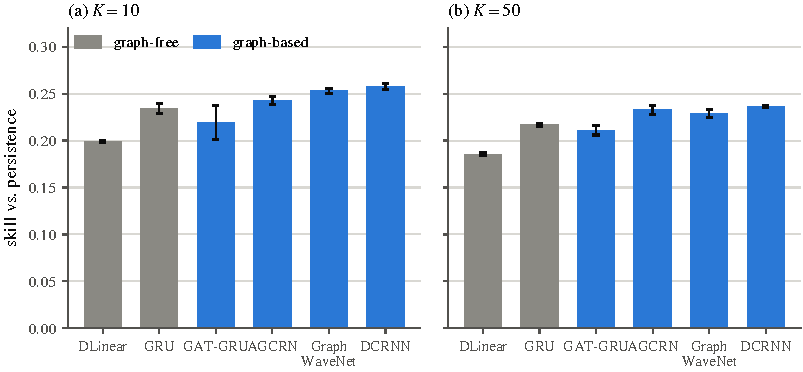
\includegraphics[width=\textwidth]{figures/fig_model_comparison.pdf}
\caption{Skill over persistence of the six learned forecasters at $K{=}10$ (left) and $K{=}50$ (right);
error bars are $\pm1$ seed std. The whole field spans only $\sim$0.06 skill: the graph models lead the
graph-free GRU by a small margin, and even a linear model is close behind.}
\label{fig:fc-compare}
\end{figure}

Three findings stand out.

\emph{First, spatial information helps --- modestly.} Every model that uses the given graph or learns one
(Graph WaveNet, DCRNN, AGCRN) beats the graph-free GRU at both sizes ($0.253$/$0.258$/$0.243$ vs.\ $0.234$
at $K{=}10$): a real, repeatable $\sim$3\% WAPE reduction. But the gain is small and does not grow with $K$,
and \emph{learning} the adjacency (AGCRN) does not beat the given Voronoi graph --- so the ceiling is the
weak residual spatial signal at cluster level, not the graph's quality. Section~\ref{sec:ablation} explains
why: the geographic aggregation has already captured most of the spatial structure, leaving little for the
inter-cluster graph to add.

\emph{Second, the field is tight and simple models lose little.} From DLinear ($0.199$) to the best model
($0.258$) the entire spread is $\sim$0.06 skill, and the no-graph GRU ($0.234$) is within $\sim$0.02 of the
best. Model choice barely moves the needle.

\emph{Third, accuracy--cost favours the simple.} DCRNN leads but is among the slowest; Graph WaveNet matches
it to within $0.005$ skill at roughly a tenth of the cost (its dilated convolutions parallelise where
DCRNN's recurrence does not); AGCRN is the costliest ($252$k parameters, $\sim$28\,min/run) for no gain; and
the in-house GAT--GRU does not lead. We therefore adopt \textbf{Graph WaveNet} as the deployed forecaster
(best accuracy--cost); a plain \textbf{GRU} would be a defensible simpler choice. The rest of the chapter
characterises Graph WaveNet, and Section~\ref{sec:ablation} shows the one decision the system is \emph{not}
insensitive to --- forecasting granularity --- dwarfs every model difference here.

\section{Effect of Cluster Count $K$}
\label{sec:graphsize}

The number of MEC clusters $K$ is a deployment parameter --- how finely the operator partitions the
city. How does the chosen forecaster (Graph WaveNet) behave as $K$ grows from a handful of clusters to
one hundred? Table~\ref{tab:fc-ksweep} sweeps $K\in\{4,\dots,100\}$ (Netflix, 3 seeds).

\begin{table}[t]
\centering
\caption{Graph WaveNet forecast quality vs.\ cluster count $K$ (Netflix, seed-averaged). Raw WAPE rises
and MAE falls with $K$ --- both intrinsic to shrinking clusters --- while \emph{skill} over the baselines
stays flat, the signature of a model that scales.}
\label{tab:fc-ksweep}
\begin{tabular}{rrrrr}
\hline
$K$ & test WAPE & test MAE & skill vs.\ persist. & skill vs.\ seasonal \\
\hline
4   & 16.4 & 0.192 & 0.266 & 0.333 \\
6   & 18.9 & 0.147 & 0.250 & 0.328 \\
8   & 20.5 & 0.120 & 0.248 & 0.329 \\
10  & 22.0 & 0.103 & 0.253 & 0.337 \\
15  & 24.8 & 0.078 & 0.239 & 0.333 \\
20  & 26.7 & 0.062 & 0.238 & 0.334 \\
30  & 30.4 & 0.048 & 0.231 & 0.335 \\
50  & 34.2 & 0.032 & 0.229 & 0.338 \\
100 & 38.8 & 0.018 & 0.232 & 0.347 \\
\hline
\end{tabular}
\end{table}

Across a $25\times$ change in $K$, Graph WaveNet holds a near-constant $\sim$0.23--0.27 skill over
persistence and $\sim$0.33 over seasonal-naive, even as raw WAPE climbs from 16.4 to 38.8 and MAE falls
from 0.192 to 0.018. The rising WAPE and falling MAE are two views of one intrinsic effect --- smaller
clusters aggregate fewer stations, so their signal is burstier in \emph{relative} terms but smaller in
\emph{absolute} terms --- while the flat skill curve shows the model keeps the same advantage regardless
of granularity (this is precisely why skill, not raw WAPE, is the headline metric). For the operator the
practical consequence is that $K$ can be chosen on deployment grounds --- number of MEC sites, controller
tractability --- without paying a forecasting penalty.

\begin{figure}[t]
\centering
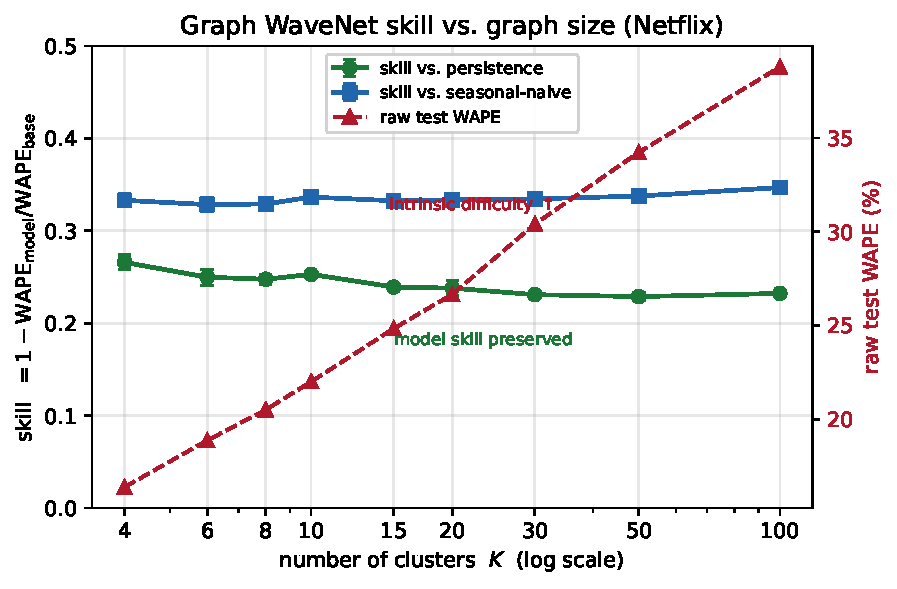
\includegraphics[width=0.78\textwidth]{figures/fig_skill_vs_k.pdf}
\caption{Graph WaveNet preserves its skill over the naive baselines from 4 to 100 clusters even as the
raw error grows with the intrinsically harder small-cluster signal. The dashed red curve (raw WAPE, right
axis) rises while the solid skill curves (left axis) stay flat.}
\label{fig:fc-skillk}
\end{figure}

\section{Generalization Across Traffic Types}
\label{sec:generalization}

Because SKATER clustering is geographic, the \emph{same} cluster structure can be re-used for a different
service, changing only the signal on the nodes. This is a clean external-validity test: does Graph WaveNet's
performance hold for traffic with a different spatial and temporal profile? Table~\ref{tab:fc-gen} reports
skill over persistence for the aggregate of all services (\texttt{total}) and the sparse \texttt{DailyMotion},
alongside Netflix, at $K\in\{8,10,15\}$ (3 seeds, frozen architecture).

\begin{table}[t]
\centering
\caption{Graph WaveNet skill over persistence by traffic type (seed-averaged). Positive for every service;
the margin tracks predictability --- largest on smooth aggregate traffic, smallest on sparse DailyMotion.}
\label{tab:fc-gen}
\begin{tabular}{lrrr}
\hline
service & $K{=}8$ & $K{=}10$ & $K{=}15$ \\
\hline
total (aggregate)   & 0.305 & 0.287 & 0.281 \\
Netflix             & 0.248 & 0.253 & 0.239 \\
DailyMotion (sparse)& 0.140 & 0.160 & 0.153 \\
\hline
\end{tabular}
\end{table}

Skill is positive for every service and every $K$, so the result is not Netflix-specific: it holds for
aggregate and sparse traffic on the same geographic graph. The margin behaves as predictability would
suggest --- widest on the smooth \texttt{total} signal ($\sim$0.29), narrower on Netflix, and smallest on
the heavily sparse DailyMotion ($\sim$0.15 vs.\ persistence). DailyMotion is the instructive case: its
persistence-skill is low because its traffic is bursty, yet its \emph{seasonal}-skill is the highest of all
($\sim$0.37) --- the sparse signal is very repetitive day-to-day, so the model beats persistence only
modestly but beats seasonal-naive strongly. The honest scope is robustness \emph{across traffic types within
Lyon}: the services share city, base stations, and period, so this is not evidence of cross-city transfer.

\begin{figure}[t]
\centering
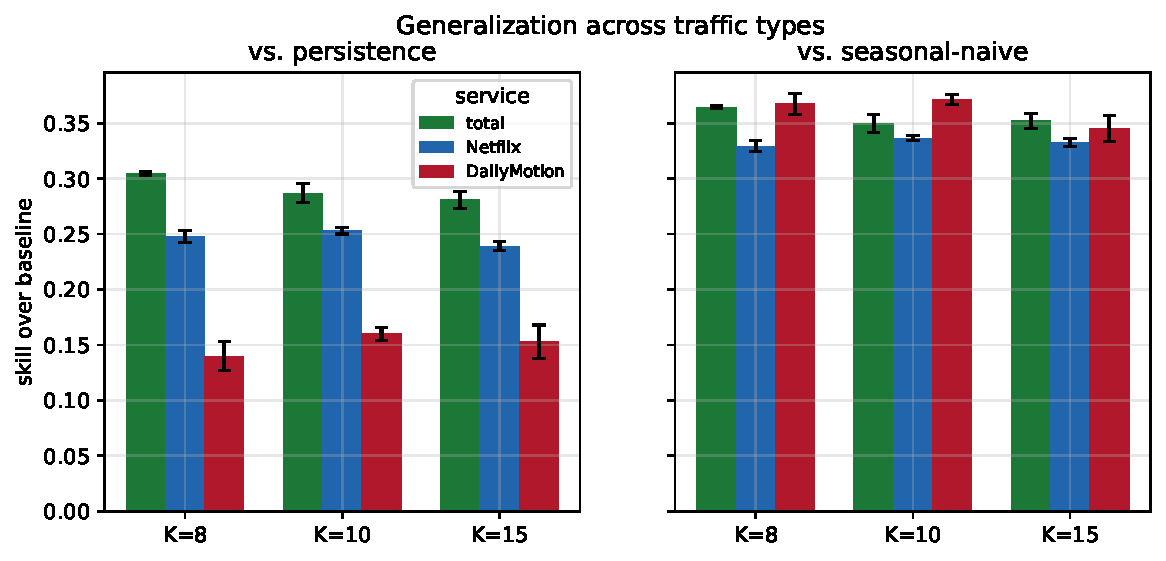
\includegraphics[width=\textwidth]{figures/fig_generalization.pdf}
\caption{Graph WaveNet's advantage over both baselines holds for aggregate and sparse traffic, scaling with
the predictability of each service. The seasonal-naive panel (right) shows DailyMotion's skill rising to
$\sim$0.37, above Netflix, despite its sparsity.}
\label{fig:fc-gen}
\end{figure}

\section{Cluster-First vs.\ Per-Base-Station: Why Aggregate?}
\label{sec:ablation}

The preceding sections chose a model (Graph WaveNet) and showed it forecasts cluster load robustly across
graph sizes and traffic types. All of it rests on one prior decision: that we forecast at the \emph{cluster}
level at all. The MEC deployment already dictates clusters --- but is aggregating first also a
\emph{forecasting} advantage, or merely a convenience we would pay for in accuracy? This closing section
tests that decision head-on.

Section~\ref{sec:graphsize} cannot answer it --- it scores each $K$ against its own (changing) target. A
controlled test instead fixes the delivered target (the $K{=}10$ cluster signal) and compares two routes to
it:
\begin{description}
  \item[Route A (cluster-first).] Aggregate to $K{=}10$ clusters; forecast the cluster signals directly.
  \item[Route B (per-base-station).] Forecast all 965 base stations; \emph{sum} the predictions into the
  same 10 clusters.
\end{description}
Both are scored on the identical $K{=}10$ target --- the 965-station series sums exactly to the cluster
series (verified to floating-point error) --- so the comparison isolates \emph{when} aggregation happens.
The route is run with the graph-free GRU and a sparse graph-attention STGNN; the dense-adjacency models
(Graph WaveNet, DCRNN, AGCRN) do not even scale to 965 nodes, which is itself telling.

\begin{figure}[t]
\centering
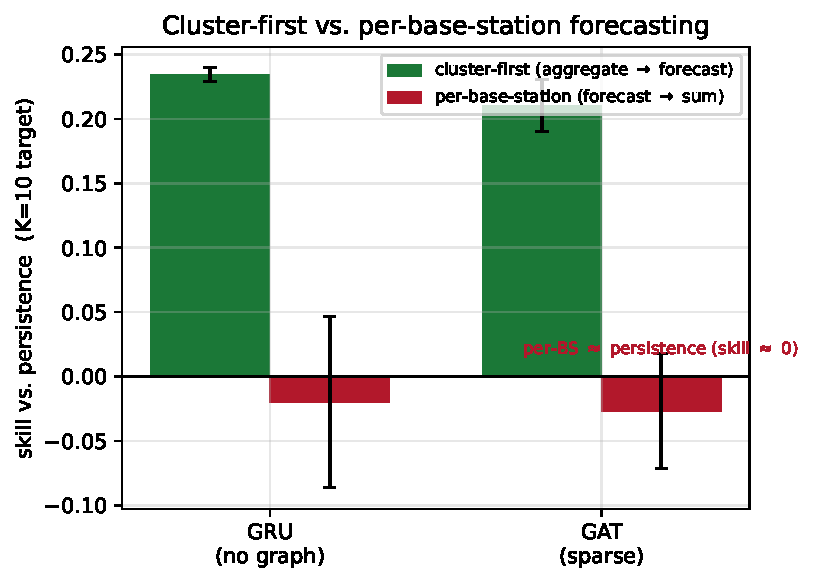
\includegraphics[width=0.68\textwidth]{figures/fig_ablation.pdf}
\caption{Forecasting the aggregated cluster signal directly (cluster-first) versus forecasting 965 base
stations and summing (per-base-station), scored on the same $K{=}10$ target. The per-station route
collapses to persistence-level skill ($\approx 0$); cluster-first reaches $0.21$--$0.23$.}
\label{fig:fc-ablation}
\end{figure}

The result (Figure~\ref{fig:fc-ablation}) is decisive: forecasting at the base-station level and summing
yields a cluster forecast \emph{no better than persistence} (skill $-0.02$ to $-0.03$), whereas forecasting
the cluster signal directly reaches $0.21$--$0.23$ --- consistent across both models and all three seeds.
The mechanism is \emph{denoising by aggregation}: per-station traffic is extremely sparse (for Netflix,
$85$--$99\%$ of station-slots are below $0.01$), so 965 such series are nearly unpredictable individually,
and a sum of persistence-level forecasts is itself persistence-level. The \emph{sum}, by contrast, is a
smooth, strongly diurnal signal that is easy to forecast.

This reframes where spatial structure helps, and closes the chapter's argument. Aggregation does not discard
spatial information --- it is the operation that \emph{exploits} it, grouping geographically coherent
stations into a predictable signal. That is why the inter-cluster graph adds only $\sim$3\% in
Section~\ref{sec:comparison} (the aggregation already did the heavy lifting), and why no model choice comes
close to the gap seen here. \textbf{Cluster-first is a forecasting advantage, not merely a tractability
convenience} --- the central, validated design decision of this chapter. (A far larger per-station model
might recover some skill, but the gap --- $0.22$ versus $\approx 0$ --- is too large to plausibly close, and
is consistent with the per-station sparsity.)

\section{Summary}
\label{sec:fc-summary}

This chapter built the spatio-temporal forecaster that supplies the digital twin's offered load.
The principal points are:

\begin{enumerate}
  \item \textbf{Scope.} The forecaster emits dimensionless per-cluster load $\hat d\in[0,1]$; physical
  calibration ($\alpha$) and control are external. One trained model serves every capacity scenario.
  \item \textbf{Cluster-first is a forecasting advantage (central result).} A controlled ablation on a
  fixed target shows that forecasting the aggregated cluster signal directly reaches $0.21$--$0.23$ skill,
  while forecasting all 965 base stations and summing is no better than persistence ($\approx 0$). The
  geographic aggregation \emph{denoises} sparse per-station traffic into a predictable signal; it is the
  operation that exploits spatial structure, not one that discards it.
  \item \textbf{Spatial structure helps modestly beyond aggregation.} On top of the clusters, the
  inter-cluster graph adds only a small gain ($\sim$3\% WAPE; graph models $>$ no-graph GRU), and a model
  that \emph{learns} its adjacency (AGCRN) does not beat the given Voronoi graph --- the residual spatial
  signal at cluster level is genuinely small.
  \item \textbf{Model choice barely matters; deploy simple.} Six forecasters from linear to learned-graph
  span only $\sim$0.06 skill; Graph WaveNet gives the best accuracy--cost trade-off and a plain GRU is
  near-best, so the system is insensitive to forecaster sophistication. Graph WaveNet is recommended for
  the twin.
  \item \textbf{The problem is well-behaved.} Skill over persistence is near-constant across graph sizes
  ($K=4\!\rightarrow\!100$; rising raw WAPE reflects intrinsic small-cluster difficulty, not model decay)
  and holds across aggregate and sparse traffic types --- evidence the findings reflect Lyon's spatial
  structure, not the Netflix trace.
\end{enumerate}

% ============================================================
%  STANDALONE-ONLY: bibliography + \end{document}.
%  Emitted only when compiling this file directly; ignored when \input into the
%  thesis (which supplies its own bibliography). Move these four entries into your
%  real thesis .bib when integrating.
% ============================================================
\ifCHFstandalone
\begin{thebibliography}{9}
\bibitem{li2018dcrnn} Y.~Li, R.~Yu, C.~Shahabi, Y.~Liu.
  Diffusion Convolutional Recurrent Neural Network: Data-Driven Traffic Forecasting.
  \emph{ICLR}, 2018.
\bibitem{wu2019gwn} Z.~Wu, S.~Pan, G.~Long, J.~Jiang, C.~Zhang.
  Graph WaveNet for Deep Spatial-Temporal Graph Modeling.
  \emph{IJCAI}, 2019.
\bibitem{bai2020agcrn} L.~Bai, L.~Yao, C.~Li, X.~Wang, C.~Wang.
  Adaptive Graph Convolutional Recurrent Network for Traffic Forecasting.
  \emph{NeurIPS}, 2020.
\bibitem{zeng2023dlinear} A.~Zeng, M.~Chen, L.~Zhang, Q.~Xu.
  Are Transformers Effective for Time Series Forecasting?
  \emph{AAAI}, 2023.
\end{thebibliography}
\end{document}
\fi
